\begin{frame}{Outliers in Linear Regression}
    \begin{itemize}
        \item We want to think about which points can be considered outliers.
        \item We also want to think about how influential these points are.
    \end{itemize}
\end{frame}

\begin{frame}{Example}
    \begin{center}
        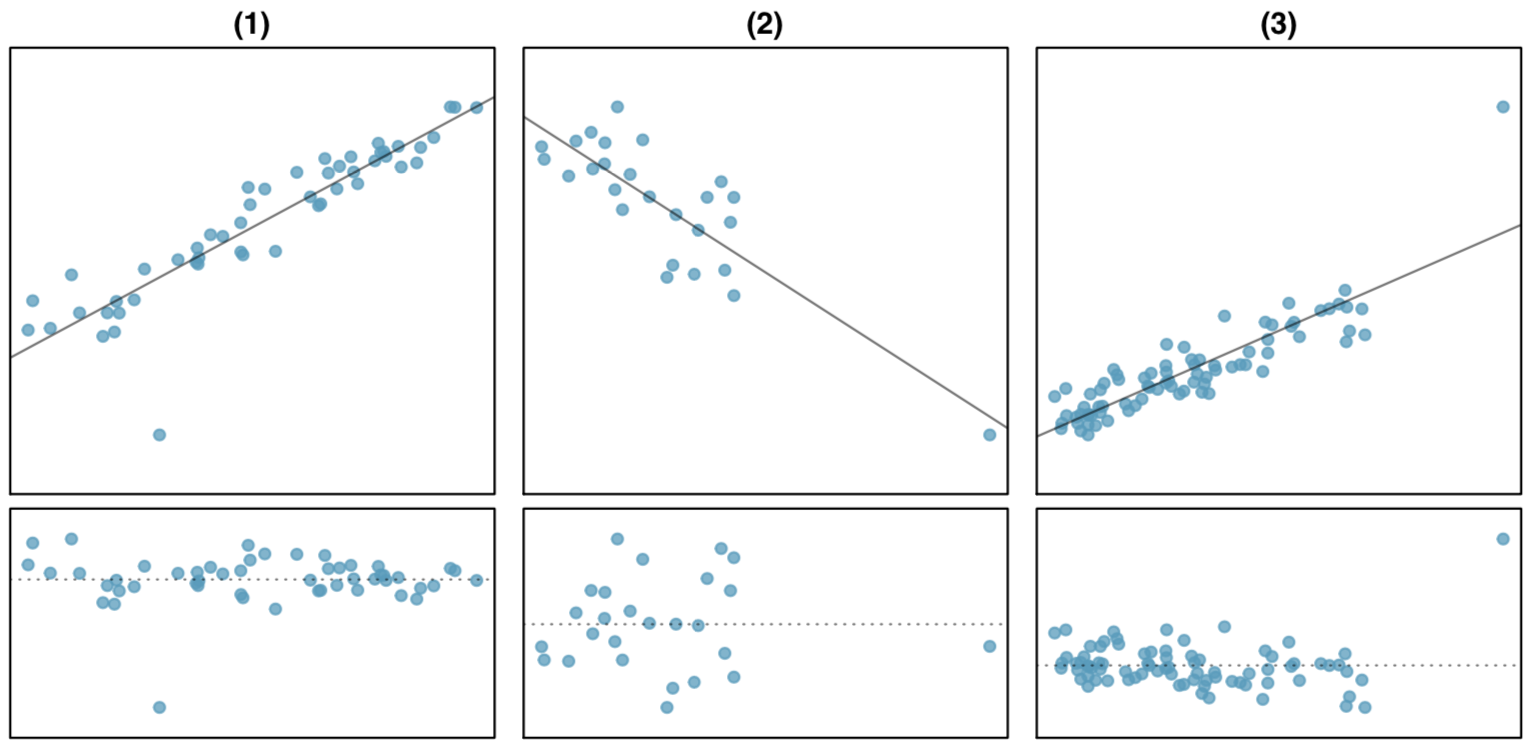
\includegraphics[width=4.5in]{images/out1.png}
    \end{center}
    %(1) There is one outlier far from the other points, though it only appears to slightly influence the line.
    %(2) There is one outlier on the right, though it is quite close to the least squares line, which suggests it wasn’t very influential.
    %(3) There is one point far away from the cloud, and this outlier appears to pull the least squares line up on the right; examine how the line around the primary cloud doesn’t appear to fit very well.
\end{frame}

\begin{frame}{Example}
    \begin{center}
        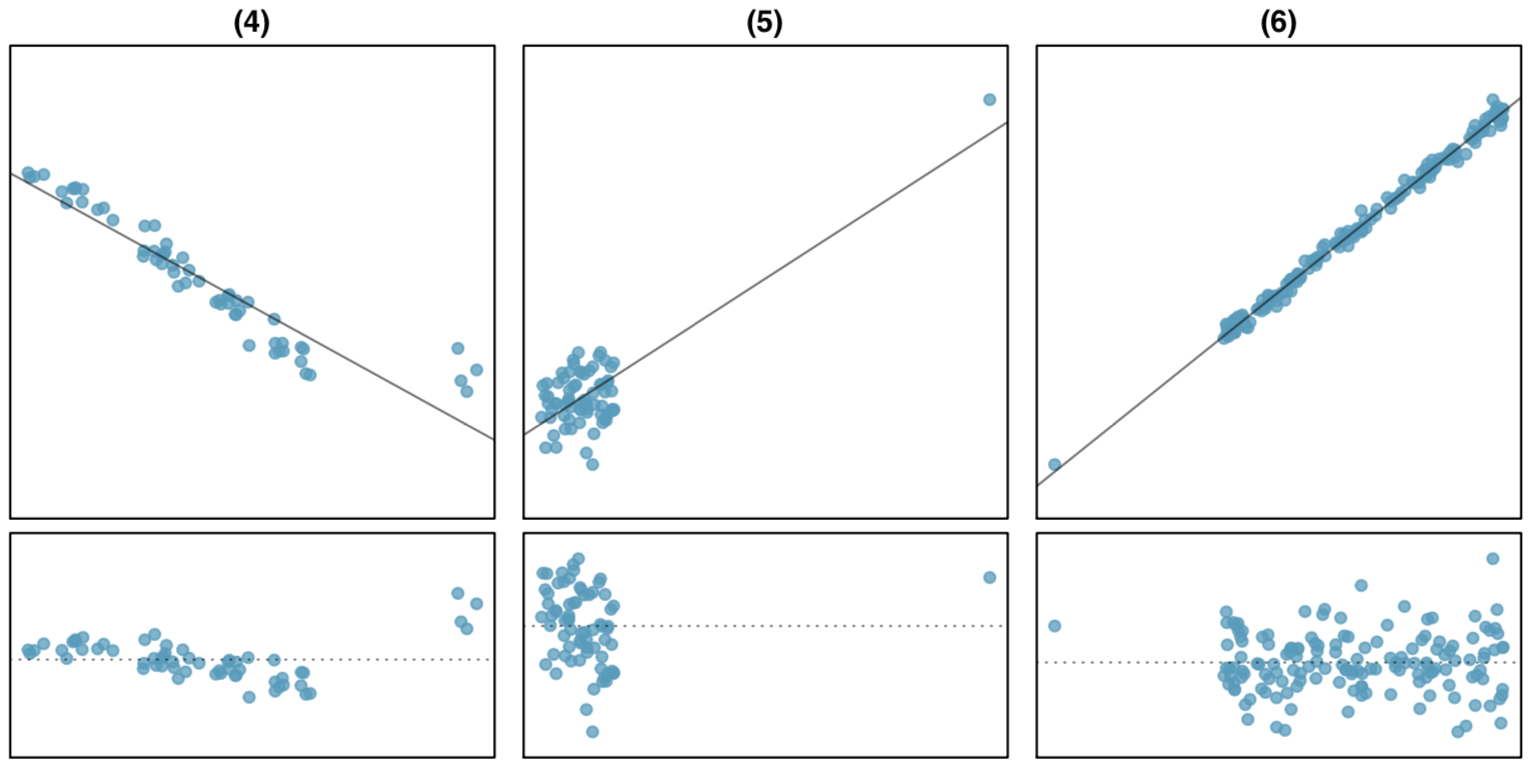
\includegraphics[width=4.5in]{images/out2.png}
    \end{center}
    %(4) There is a primary cloud and then a small secondary cloud of four outliers. The secondary cloud appears to be influencing the line somewhat strongly, making the least square line fit poorly almost everywhere. There might be an interesting explanation for the dual clouds, which is something that could be investigated.
    %(5) There is no obvious trend in the main cloud of points and the outlier on the right appears to largely control the slope of the least squares line.
    %(6) There is one outlier far from the cloud. However, it falls quite close to the least squares line and does not appear to be very influential.
\end{frame}

\begin{frame}{Leverage}
    Points that fall away horizontally from the center of the cloud tend to pull harder on the line. We refer to these points as \textbf{high leverage}.
\end{frame}

\begin{frame}{Influential Points}
    \begin{itemize}
        \item We conclude that a point is \textbf{influential} if, had we fit the line without it
        \begin{itemize}
            \item the line would have been very different.
            \item the point would have been far from the line.
        \end{itemize}
    \end{itemize}
\end{frame}

\begin{frame}{Example}
    \begin{center}
        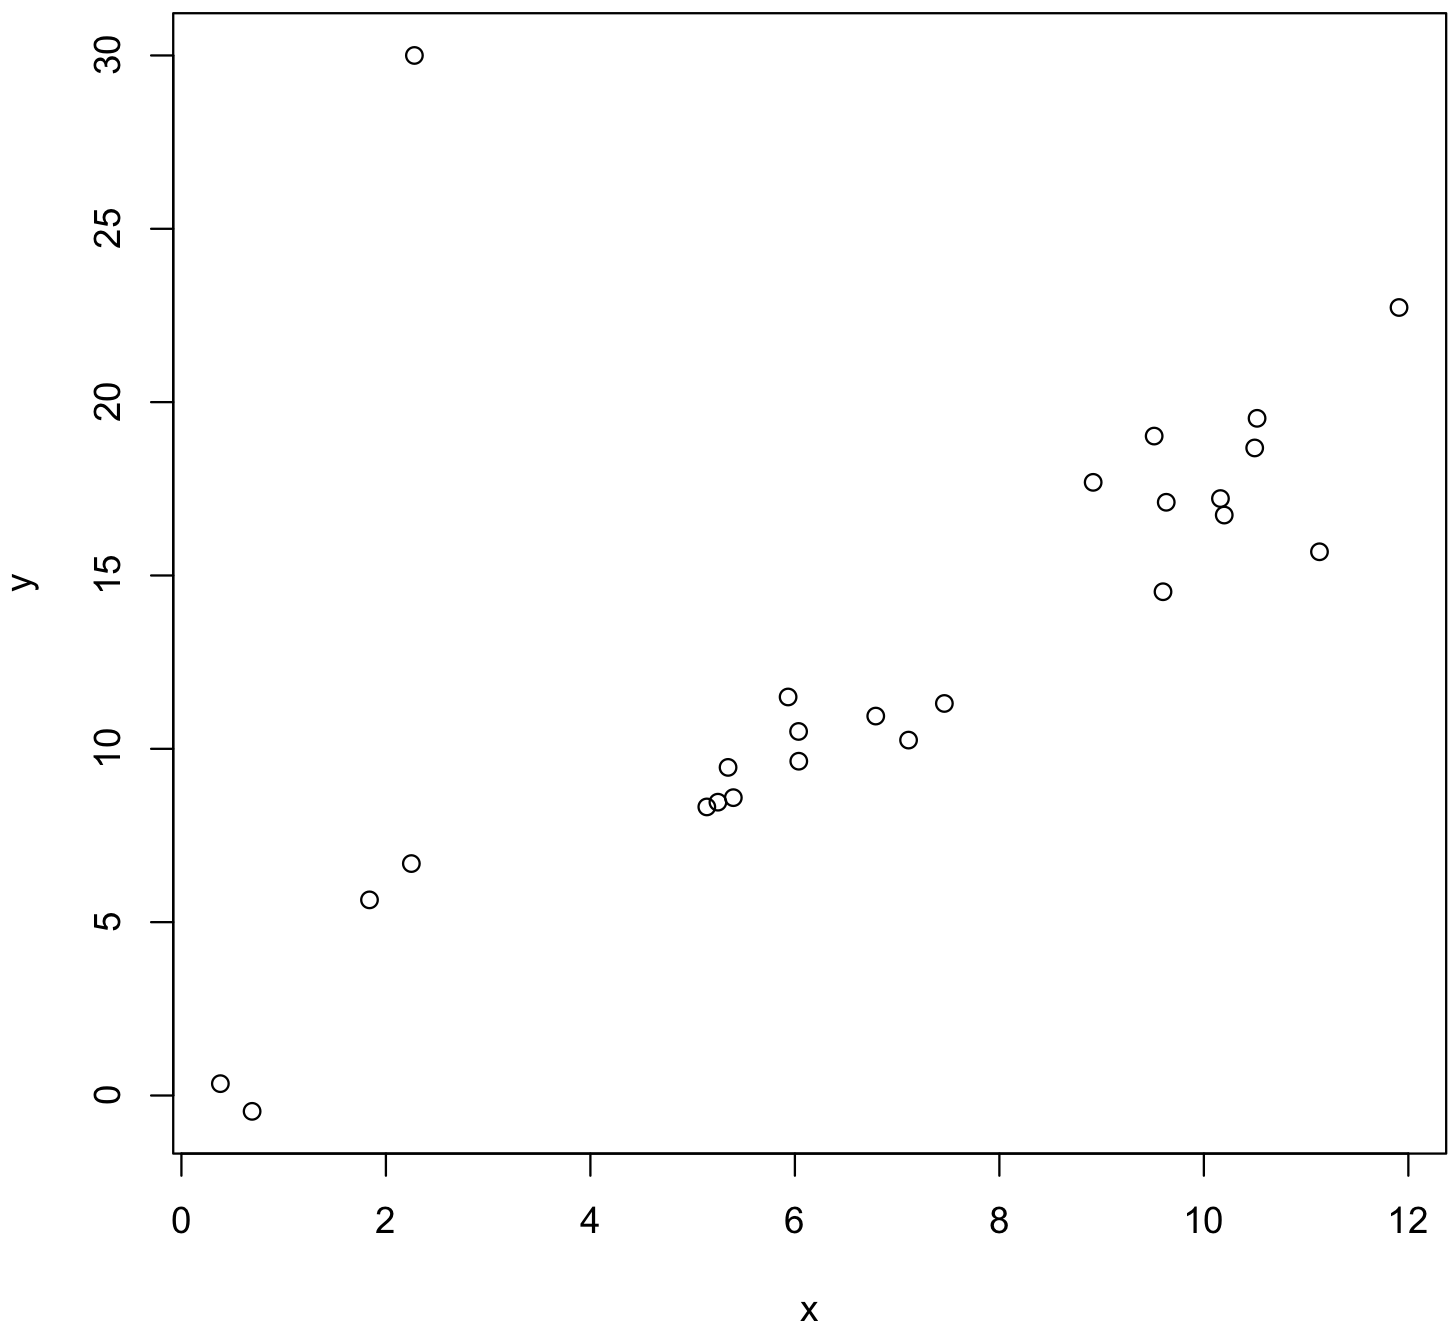
\includegraphics[height=3in]{images/outlier.png}
    \end{center}
\end{frame}

\begin{frame}{Example}
    \begin{center}
        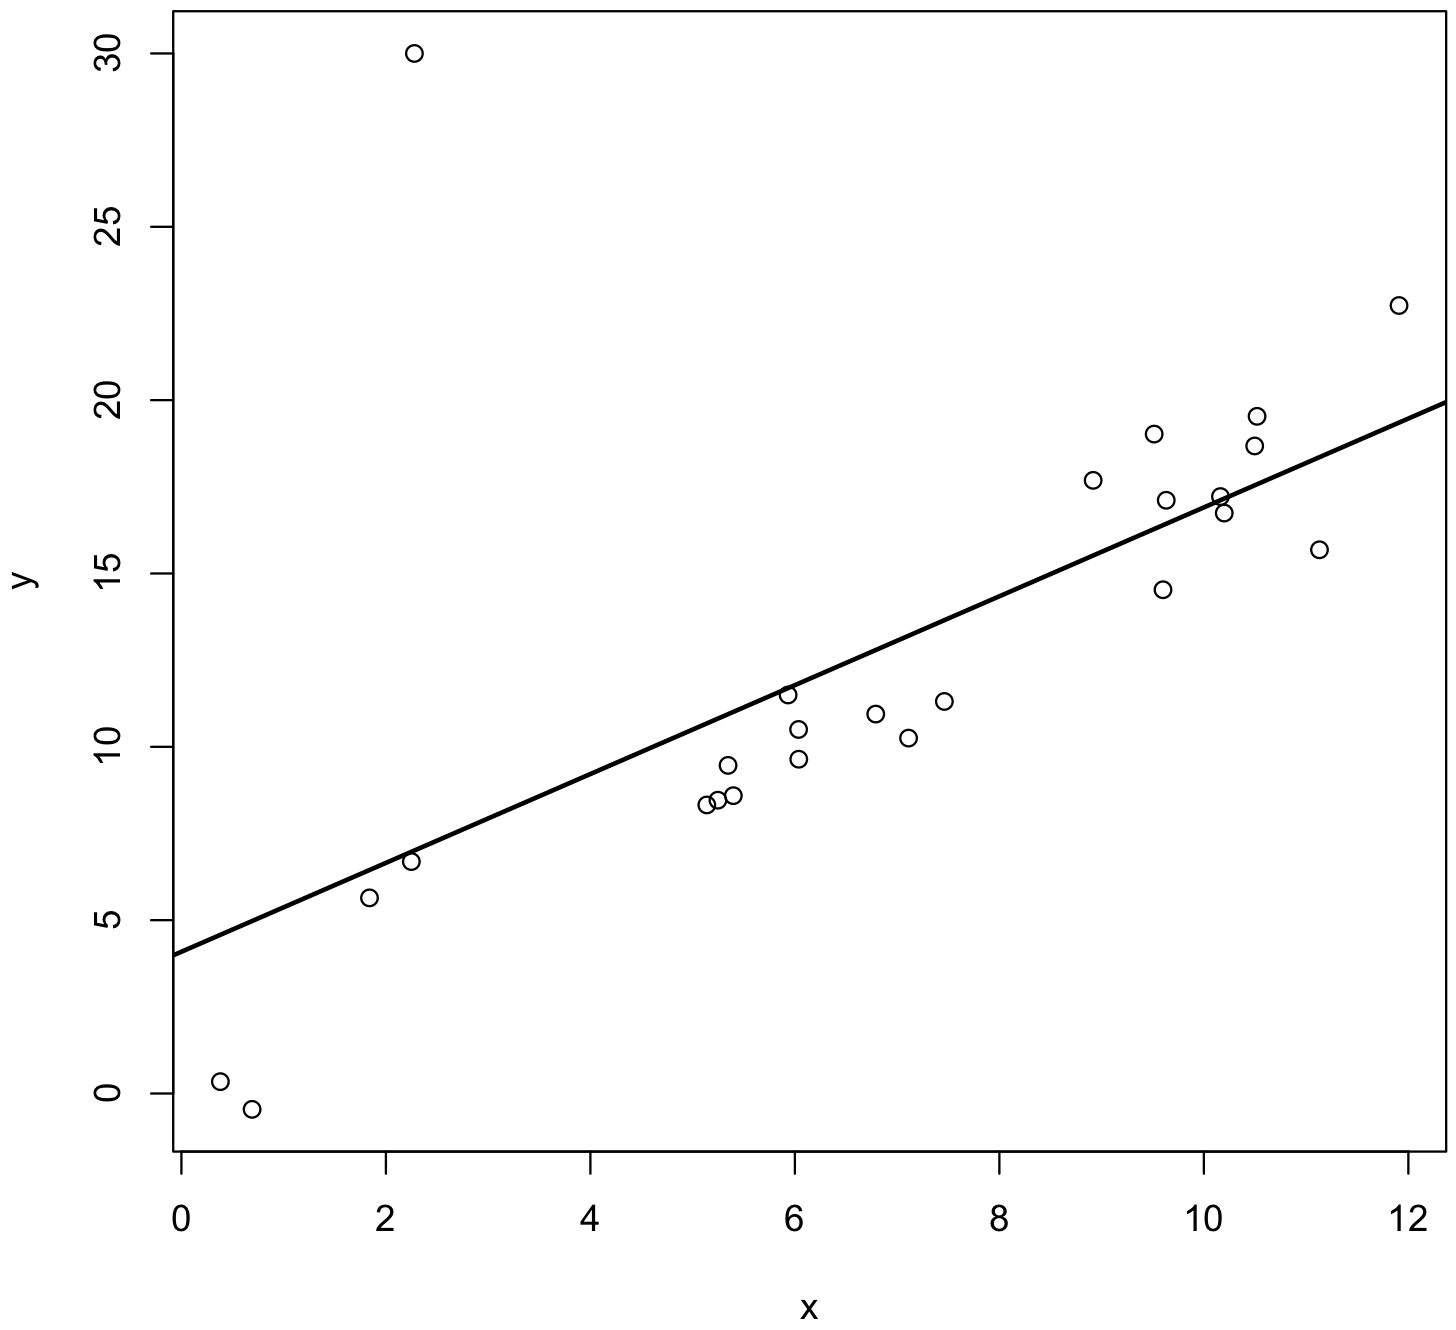
\includegraphics[height=2.5in]{images/outlierline.png}
    \end{center}
    \vspace{-0.5cm}The least squares regression line is $\hat{y} = 4.0886 + 1.2817x$.
\end{frame}

\begin{frame}{Example}
    If we remove this point and rerun the regression, we get the line
    \[
        \hat{y} = 0.1923 + 1.7021x
    \]
    a significant deviation from the original line,
    \[
        \hat{y} = 4.0886 + 1.2817x
    \]
\end{frame}

\begin{frame}{Example}
    \begin{center}
        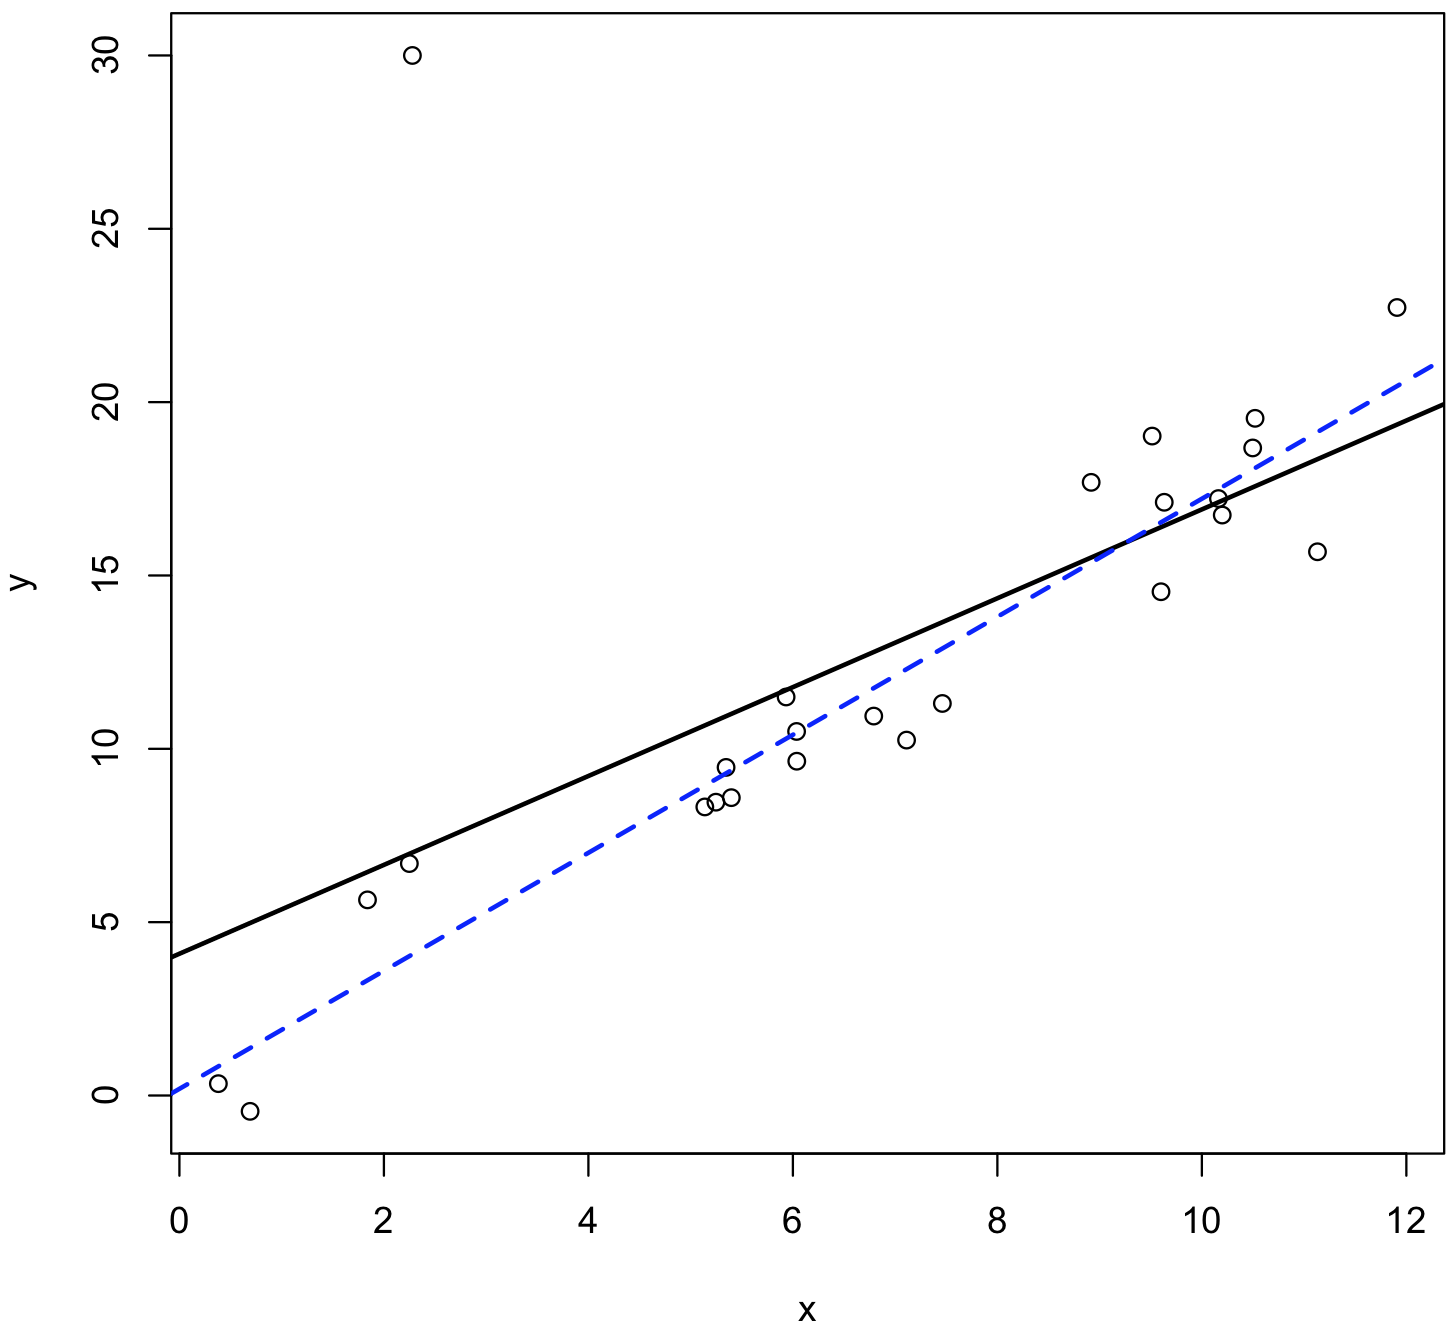
\includegraphics[height=2.5in]{images/outlier2lines.png}
    \end{center}
    \vspace{-0.5cm}The blue dashed line is the regression line with the extreme point removed.
\end{frame}

\begin{frame}{Example}
    I actually simulated 25 data points under
    \[
        y = 2 + 1.5x + \epsilon
    \]
    and then changed one of the points to create an outlier.
\end{frame}

\begin{frame}{Example}
    \begin{center}
        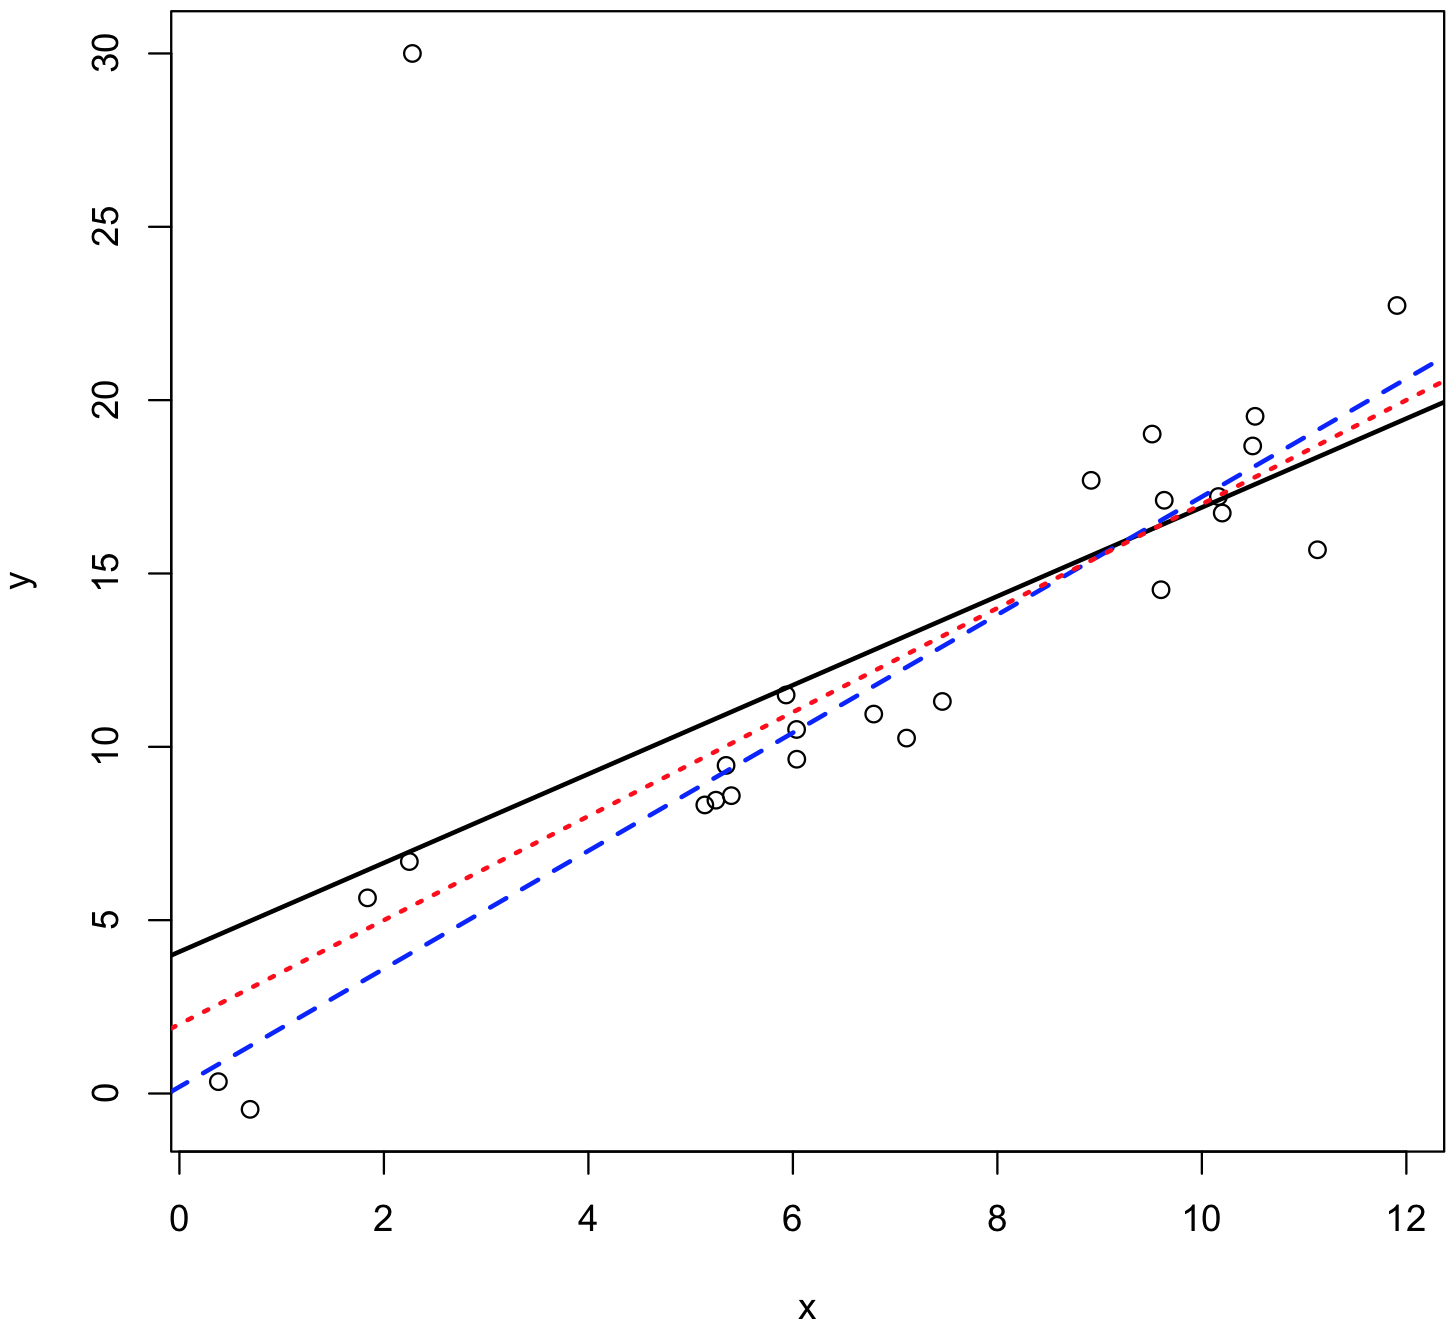
\includegraphics[height=2.5in]{images/outlier3lines.png}
    \end{center}
    \vspace{-0.5cm}The red dotted line is the truth.
\end{frame}

\begin{frame}{Diagnosing Problematic Points}
    \vspace{-0.5cm}\begin{center}
        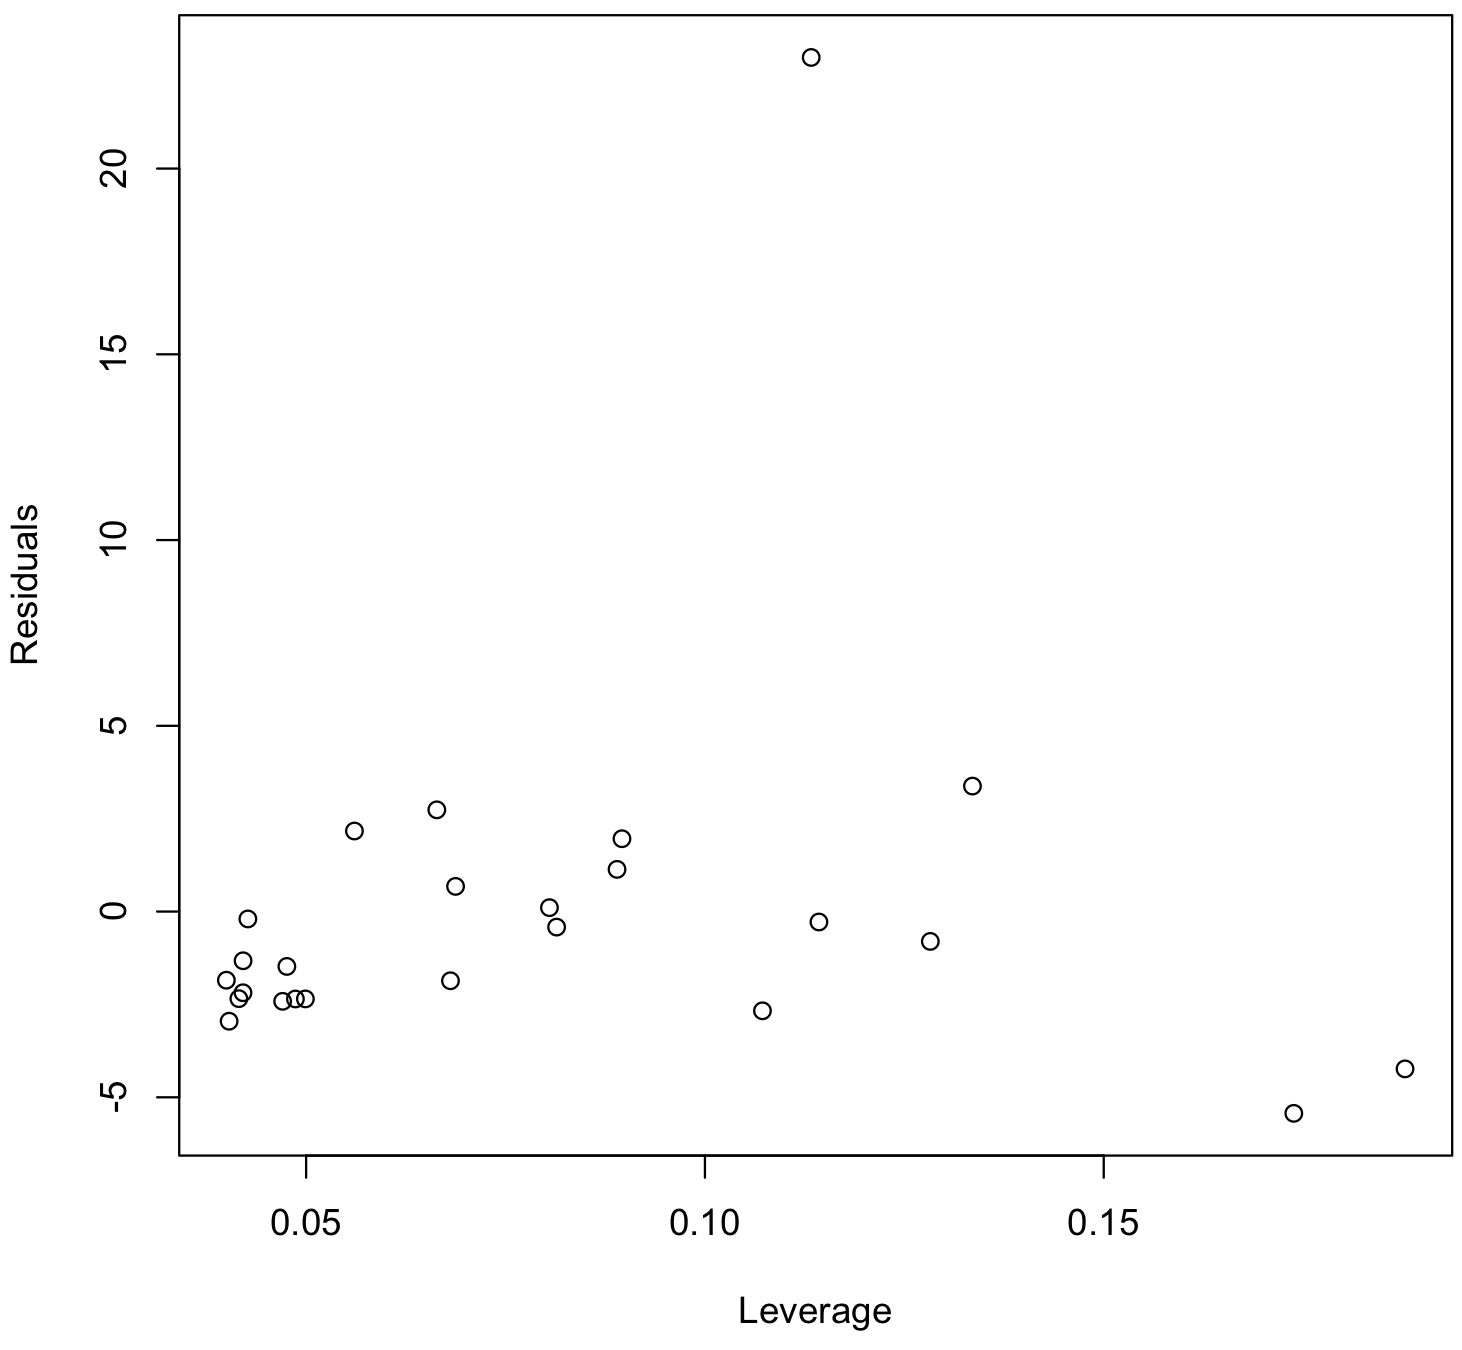
\includegraphics[height=2.5in]{images/reslev.png}
    \end{center}
    We are interested in points with high leverage \textit{and} extreme residuals.
\end{frame}

\begin{frame}{Cook's Distance}
    \begin{itemize}
        \item We're not too concerned about outliers if they are low leverage.
        \item We're also not too concerned about high leverage points if they are not outliers.
        \item When is a point an outlier and high leverage? Enter Cook's distance.
    \end{itemize}
\end{frame}

\begin{frame}{Residuals vs Leverage}
    \vspace{-0.5cm}\begin{center}
        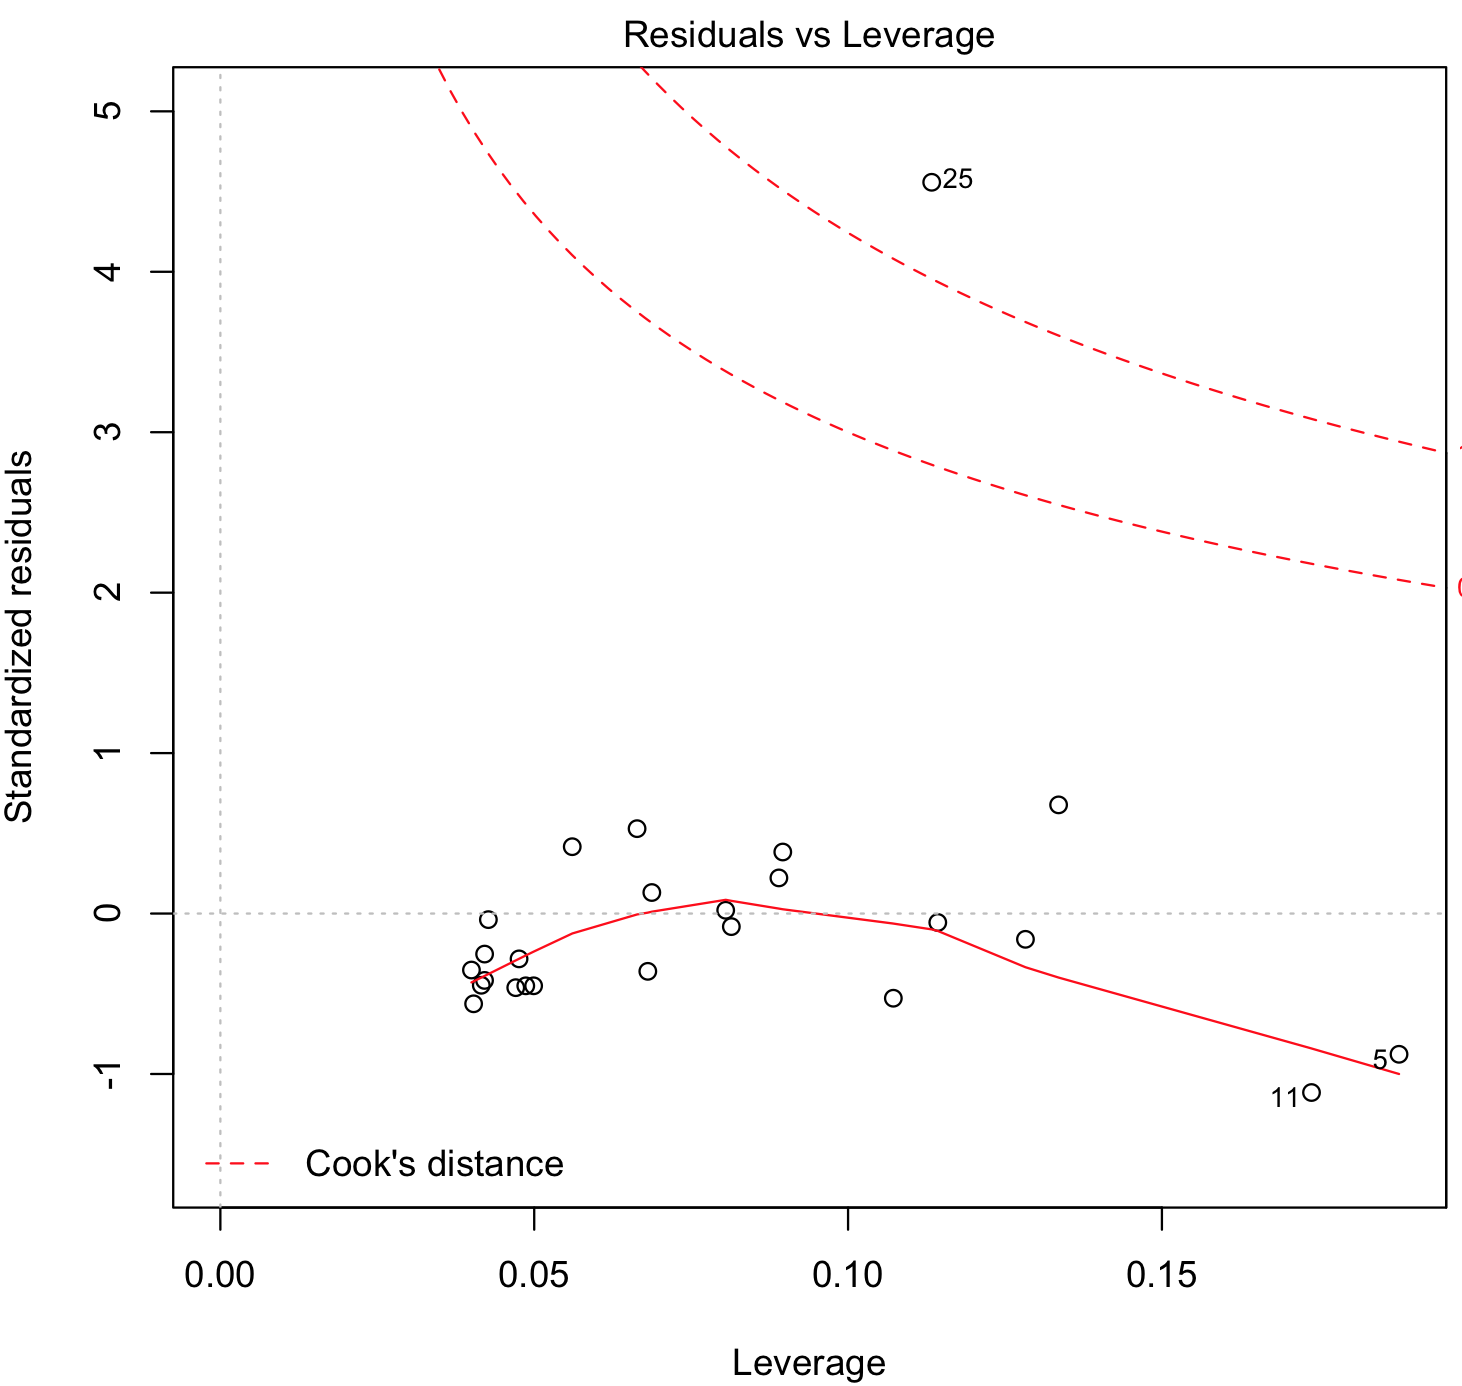
\includegraphics[height=2.5in]{images/residlev.png}
    \end{center}
    This is the final diagnostic plot automatically generated by R.
\end{frame}

\begin{frame}{Removing Outliers}
    \begin{itemize}
        \item It may be temping to remove outliers.
        \item However, we don't want to remove outliers for purely mathematical reasons!
        \item Outliers should be removed for good scientific reasons.
        \begin{itemize}
            \item Faulty equipment, mis-entered data, etc.
        \end{itemize}
        \item Sometimes outliers are the most interesting part of the data!
    \end{itemize}
\end{frame}
